%%%%%%%%%%%%%%%%%%%%%%%%%%%%%%%%%%%%%%%%%
% Arsclassica Article
% LaTeX Template
% Version 1.1 (10/6/14)
%
% This template has been downloaded from:
% http://www.LaTeXTemplates.com
%
% Original author:
% Lorenzo Pantieri (http://www.lorenzopantieri.net) with extensive modifications by:
% Vel (vel@latextemplates.com)
%
% License:
% CC BY-NC-SA 3.0 (http://creativecommons.org/licenses/by-nc-sa/3.0/)
%
%%%%%%%%%%%%%%%%%%%%%%%%%%%%%%%%%%%%%%%%%

%----------------------------------------------------------------------------------------
%	PACKAGES AND OTHER DOCUMENT CONFIGURATIONS
%----------------------------------------------------------------------------------------

\documentclass[
10pt, % Main document font size
a4paper, % Paper type, use 'letterpaper' for US Letter paper
oneside, % One page layout (no page indentation)
%twoside, % Two page layout (page indentation for binding and different headers)
headinclude,footinclude, % Extra spacing for the header and footer
BCOR5mm, % Binding correction
]{scrartcl}

%%%%%%%%%%%%%%%%%%%%%%%%%%%%%%%%%%%%%%%%%
% Arsclassica Article
% Structure Specification File
%
% This file has been downloaded from:
% http://www.LaTeXTemplates.com
%
% Original author:
% Lorenzo Pantieri (http://www.lorenzopantieri.net) with extensive modifications by:
% Vel (vel@latextemplates.com)
%
% License:
% CC BY-NC-SA 3.0 (http://creativecommons.org/licenses/by-nc-sa/3.0/)
%
%%%%%%%%%%%%%%%%%%%%%%%%%%%%%%%%%%%%%%%%%

%----------------------------------------------------------------------------------------
%	REQUIRED PACKAGES
%----------------------------------------------------------------------------------------

\usepackage[
nochapters, % Turn off chapters since this is an article        
beramono, % Use the Bera Mono font for monospaced text (\texttt)
eulermath,% Use the Euler font for mathematics
pdfspacing, % Makes use of pdftex’ letter spacing capabilities via the microtype package
dottedtoc % Dotted lines leading to the page numbers in the table of contents
]{classicthesis} % The layout is based on the Classic Thesis style

\usepackage{arsclassica} % Modifies the Classic Thesis package

\usepackage[T1]{fontenc} % Use 8-bit encoding that has 256 glyphs

\usepackage[utf8]{inputenc} % Required for including letters with accents

\usepackage{graphicx} % Required for including images
\graphicspath{{Figures/}} % Set the default folder for images

\usepackage{enumitem} % Required for manipulating the whitespace between and within lists

\usepackage{lipsum} % Used for inserting dummy 'Lorem ipsum' text into the template

\usepackage{subfig} % Required for creating figures with multiple parts (subfigures)

\usepackage{amsmath,amssymb,amsthm} % For including math equations, theorems, symbols, etc

\usepackage{varioref} % More descriptive referencing



%----------------------------------------------------------------------------------------
%	THEOREM STYLES
%---------------------------------------------------------------------------------------

\theoremstyle{definition} % Define theorem styles here based on the definition style (used for definitions and examples)
\newtheorem{definition}{Definition}

\theoremstyle{plain} % Define theorem styles here based on the plain style (used for theorems, lemmas, propositions)
\newtheorem{theorem}{Theorem}

\theoremstyle{remark} % Define theorem styles here based on the remark style (used for remarks and notes)

%----------------------------------------------------------------------------------------
%	HYPERLINKS
%---------------------------------------------------------------------------------------

\hypersetup{
%draft, % Uncomment to remove all links (useful for printing in black and white)
colorlinks=true, breaklinks=true, bookmarks=true,bookmarksnumbered,
urlcolor=webbrown, linkcolor=RoyalBlue, citecolor=webgreen, % Link colors
pdftitle={}, % PDF title
pdfauthor={\textcopyright}, % PDF Author
pdfsubject={}, % PDF Subject
pdfkeywords={}, % PDF Keywords
pdfcreator={pdfLaTeX}, % PDF Creator
pdfproducer={LaTeX with hyperref and ClassicThesis} % PDF producer
}

 % Include the structure.tex file which specified the document structure and layout

\usepackage{listings}

\hyphenation{Fortran hy-phen-ation} % Specify custom hyphenation points in words with dashes where you would like hyphenation to occur, or alternatively, don't put any dashes in a word to stop hyphenation altogether

%----------------------------------------------------------------------------------------
%	TITLE AND AUTHOR(S)
%----------------------------------------------------------------------------------------

\title{ISS Project: MortgageConversionAndLoan Service} % The article title

\author{\spacedlowsmallcaps{Menelaos Ralli Camara}} % The article author(s) - author affiliations need to be specified in the AUTHOR AFFILIATIONS block

\date{29 January 2016} % An optional date to appear under the author(s)

%----------------------------------------------------------------------------------------

\lstset{language = XML,
		basicstyle = \small,
		escapeinside={(*@}{@*)},  }
\newcommand{\xmlscript}[2]{
\lstinputlisting[caption=#2,label=#1]{#1.xml}
} 

\def\restsource{\url{http://currencyconverter.kowabunga.net/converter}\ }
\def\mortgageservice{\url{http://www.webservicex.net/mortgage.asmx?WSDL}\ }
\def\financeservice{\url{http://www.webservicex.net/FinanceService.asmx?WSDL}\ }
\begin{document}

%----------------------------------------------------------------------------------------
%	HEADERS
%----------------------------------------------------------------------------------------

\renewcommand{\sectionmark}[1]{\markright{\spacedlowsmallcaps{#1}}} % The header for all pages (oneside) or for even pages (twoside)
%\renewcommand{\subsectionmark}[1]{\markright{\thesubsection~#1}} % Uncomment when using the twoside option - this modifies the header on odd pages
\lehead{\mbox{\llap{\small\thepage\kern1em\color{halfgray} \vline}\color{halfgray}\hspace{0.5em}\rightmark\hfil}} % The header style

\pagestyle{scrheadings} % Enable the headers specified in this block

%----------------------------------------------------------------------------------------
%	TABLE OF CONTENTS & LISTS OF FIGURES AND TABLES
%----------------------------------------------------------------------------------------

\maketitle % Print the title/author/date block

\setcounter{tocdepth}{2} % Set the depth of the table of contents to show sections and subsections only

\tableofcontents % Print the table of contents

\listoffigures % Print the list of figures

\newpage % Start the article content on the second page, remove this if you have a longer abstract that goes onto the second page

%----------------------------------------------------------------------------------------
%	INTRODUCTION
%----------------------------------------------------------------------------------------

\section{Introduction}
MortgageConversionAndLoan is a service which provide the total monthly
mortgage converted from one currency to another and the monthly loan.
More in detail the service provide the getMortgageConversionAndLoan SOAP operation
that take as an input the following parameters:
\begin{itemize}

\item \textbf{MortgageYears}: Total duration of the mortgage in years
\item \textbf{MortgageInterest}: Interest rate of the mortgage
\item \textbf{MortgageLoanAmount}: Total amount of the loan
\item \textbf{MortgageAnnualTa}: Possible annual taxes to be paid
\item \textbf{MortgageAnnualInsurance}: Possible annual insurances to be paid
\item \textbf{CurrencyFrom}: The currency to be converted
\item \textbf{CurrencyTo}: The currency in which to convert the mortgage
\item \textbf{LoanAmount}: Total Loan amount
\item \textbf{InterestRate} : Interest rate of the loan
\item \textbf{Months}: Total duration of the loan in months

\end{itemize}
As result, the service sends back to the client the following response:

\begin{itemize}
\item \textbf{MortgageTotalAmountConverted}: Monthly mortgage converted
\item \textbf{MonthlyTaxRate}: Monthly tax rate to be paid
\item \textbf{MonthlyInsuranceRate}: Monthly insurance rate to be paid
\item \textbf{LoanMonthlyPaymentResult}: Monthly loan to be paid
\end{itemize}

This service uses the following three external services to compose the
response:

\begin{itemize}

\item \textbf{LOAN / APR / Lease} (later on A) a REST and SOAP service that provide
different operations including the LoanMonthlyPayment operation
which given the total loan amount the interest rate and the duration
it returns the monthly loan to be pay. The orchestrator uses
the LoanMonthlyPayment SOAP operation described in the WSDL
(\financeservice) of A
\item \textbf{Mortgage Web service} (Later on B) a REST and SOAP service that retrieves
the monthly mortgage amount free from taxes and insurance,
the monthly amount of taxes and insurance and the total monthly
mortgage amount including taxes and insurance. The orchestrator
uses the GetMortgagePayment SOAP operation, described in the WSDL
(\mortgageservice) of B
\item \textbf{CurrencyConverter} (Later on C) a REST and SOAP service which provides
different operations including the GetConversionAmount that
retrieves the currency conversion of a given amount from one currency
to another. The orchestrator exploit to convert the total monthly mortgage
amount by means of this REST resource: \restsource.

\end{itemize}


The relation between input and output is illustrated in figure \ref{fig:IORelations}

\begin{figure}[tb]
\centering
\subfloat[Flow1 IO relation]{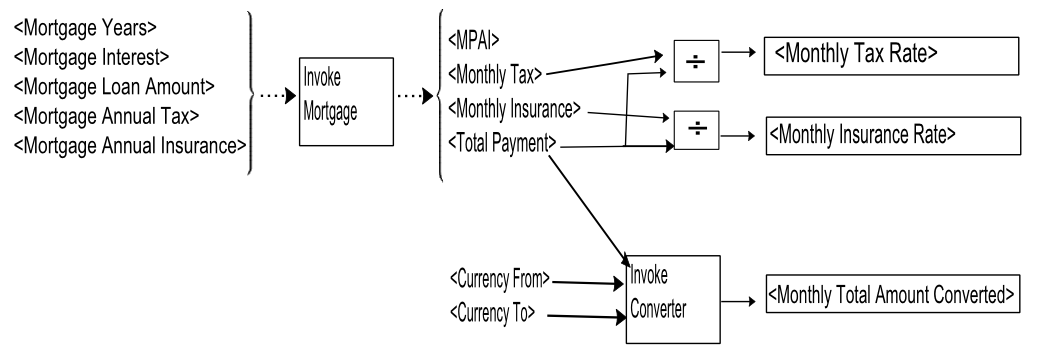
\includegraphics[width=1\columnwidth]{./pictures/IORelationFlow1.png}} \quad
\subfloat[Flow2 IO relation]{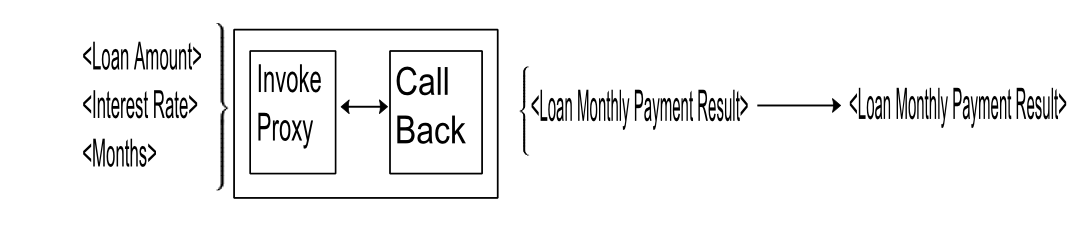
\includegraphics[width=1\columnwidth]{./pictures/IORelationFlow2.png}} \\
\caption[IO Relations]{} % The text in the square bracket is the caption for the list of figures while the text in the curly brackets is the figure caption
\label{fig:IORelations}
\end{figure}

The figure \ref{fig:Scheme} illustrates a sketch of the application structure
\begin{figure}[tb]
\centering 
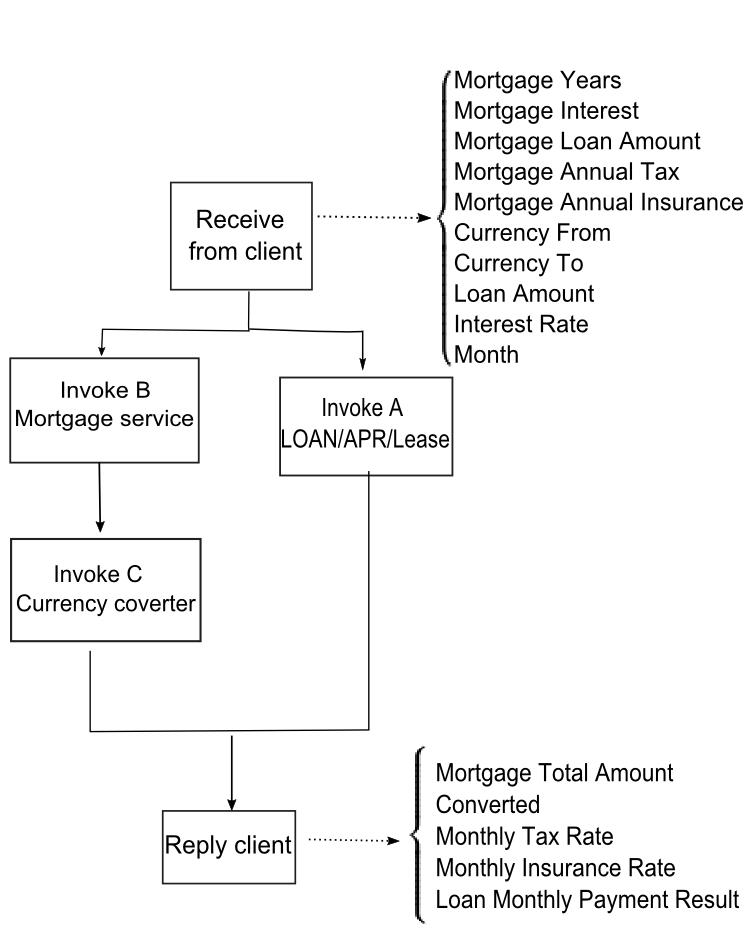
\includegraphics[width=1\columnwidth]{./pictures/APIScheme.png} 
\caption[Application Structure]{Application structure}  % The text in the square bracket is the caption for the list of figures while the text in the curly brackets is the figure caption
\label{fig:Scheme} 
\end{figure}

%----------------------------------------------------------------------------------------
%	WS-BPEL IMPLEMENTATION
%----------------------------------------------------------------------------------------

\section{WS-BPEL IMPLEMENTATION}

The WS-BPEL of the service orchestrator is composed of two parts, the
MortgageConversionLoanService, which perform the real orchestration of the external
services and the LoanAmountProxyCA that is a service proxy that
asynchronously calls the service A, which does not provide itself an asynchronous
interface. The proxy only sends back all the responses from A to
the caller. Particular attention was taken in developing the callback mechanism
of the proxy in such a way that its responses also contained the original
input, thus enabling the orchestrator to create a correlation between the
asynchronous invocation and the callback result.

\subsection{WS-BPEL processes}
To compute its answer message the orchestrator executes concurrently to
tasks. On one hand, service B is called to retrieve the monthly mortgage
amount and the monthly mortgage tax an insurance to be pay, afterwards a
call of service C convert the monthly mortgage amount from one currency
to another. On the other hand, the parallel invocation of service A asynchronously
call of the service A gets the monthly loan amount to be paid.


At this point, we can have different outcomes: - if the callback message
is not received within a time window of 10 seconds, the service throws
a to\_fault error, the process is aborted and the fault is forwarded to the
client; - if the callback message comes before the timeout, the message is
parsed, the LoanMonthlyPayementResult is obtained. 

If any error shows up during the parsing of the callback response, then a Loan\_reply\_fault is
thrown without interrupting the flow of the process but simply replying
an error code instead loan monthly payment, i.e. the client will only receive
the the total mortgage monthly payment converted and the monthly tax rate
and the monthly insurance rate.


If any error shows up during the parsing of B response the a Mortgage\_reply\_fault
is thrown without interrupting the other parallel flow, i.e the client will only
receive the LoanMonthlyPaymentResult.


This behaviour is implemented employing three scopes and three different
fault handlers respectively. Particularly there are the ExternalScope
scope that covers the whole service, the LoanScope scope that covers the
flow sequence with the invocation to A and the MortgageScope that covers
the flow sequence with the B and C invocation. So when the to\_fault fault
is thrown, the fault handler in the ExternalScope catches it and the execution
of the process is interrupted; otherwise when the Mortgage\_reply\_fault
or Loan\_reply\_fault is thrown, respectively the fault handler in the MortgageScope
and in the LoanScope catches it. In figure \ref{fig:Scope} is illustrated the structure of the WS-BPEL scopes

\begin{figure}[tb]
\centering 
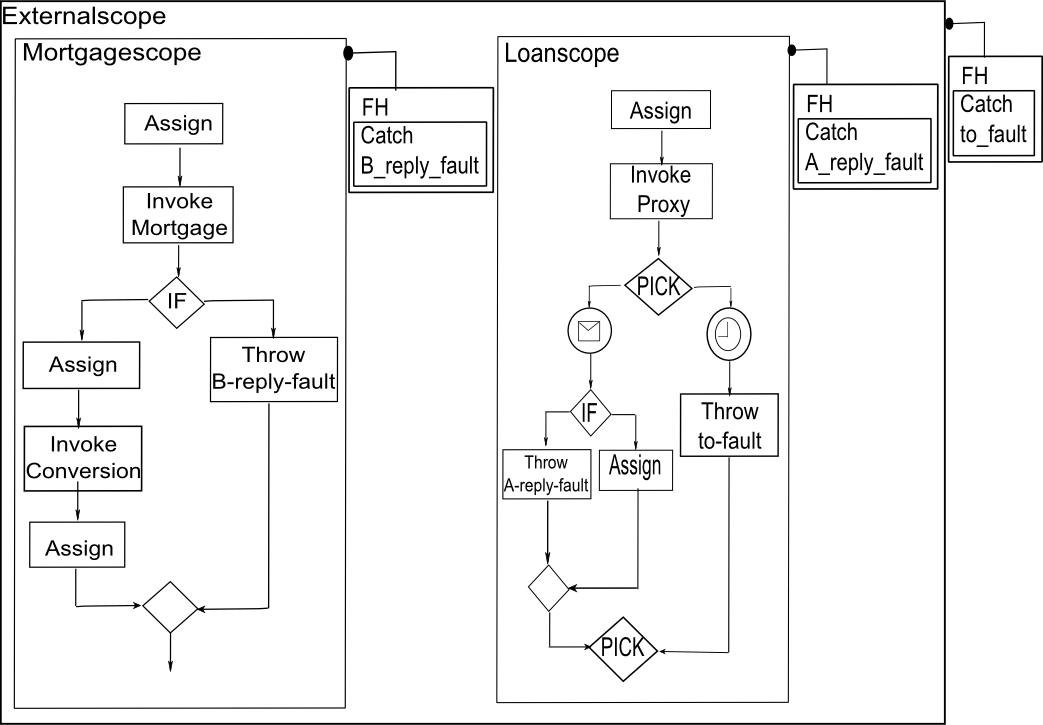
\includegraphics[width=1\columnwidth]{./pictures/APIScope.png} 
\caption[WS-BPEL Scopes]{WS-BPEL Scopes and the respective fault handlers}  
\label{fig:Scope} 
\end{figure}

\subsection{Test}

To test the MortgageConversionAndLoan Service five types of test were designed.
The former two contain the correct results of standard invocation,
the latter three possible faulty calls.
Below the tests correct1 and correct2 are listed:

\xmlscript{./code/correct1}{}
\xmlscript{./code/correct2}{}

Among all the possible wrong input the following one is used to trigger
the Mortgage\_reply\_fault error:

\xmlscript{./code/mortgagefault}{}

In this case, the received response is composed of an error message for
the MortgageTotalAmountConverted tag and NaN message for the MonthlyTaxRate
and MonthlyInsuranceRate tag instead the LoanMonthlyPaymentResult
tag is not affected by this fault hence it looks like:

\xmlscript{./code/mortgagefaultresponse}{}

Among all the possible wrong input the following one is used to trigger
the Loan\_reply\_fault error:

\xmlscript{./code/loanfault}{}

In this case, the received response is composed of an error message for
the LoanMonthlyPaymentResult whereas the other tags are not affected by
this fault, hence it looks like:

\xmlscript{./code/loanfaultresponse}{}

The most tricky test is the one for the to\_fault, having to introduce a delay
in the asynchronous answer of the proxy in such a way that the timeout of
10 seconds is exceeded. For this reason by adding a wait command in the
WS-BPEL of the proxy before the invocation we get the following output:

\xmlscript{./code/timeoutfaultresponse}{}


%----------------------------------------------------------------------------------------
%	analysis of the ws-bpel specification
%----------------------------------------------------------------------------------------


\section{ANALYSIS OF THE WS-BPEL SPECIFICATION}


The control flow of the main WS-BPEL process is also implemented through
a workflow net, and thanks to the WoPeD software it is also proved sound.
Actually this does not guarantee that the orchestrator always works as expected,
nevertheless it is indeed a good result, from a modeling point of
view.
The more difficult part in the implementation of the workflow net is the
error handling of the three kinds of faults. Whereas the Loan\_reply\_fault
and Mortgage\_reply\_fault are handled easily – adding a XOR-join transition
at the end of the flow in such a way the answer is build correctly either or
with out the error message – because it does not disrupt the flow of the
process.
On the other hand the to\_fault must interrupt the execution of the other
parallel flow no matter in which place the related token is, i.e. either if no invocation
are done yet, if only the invocation to service B or both invocation
are done. The only exception for the interrupt of the execution is in which
the Mortgage\_reply\_fault handler is already started. Indeed in this situation
the already active fault handling is allowed to complete. Furthermore
although in the WS-BPEL specification the if condition MUST be terminated
immediately in the workflow model the if condition is not terminated immediately,
this choice will not have any impact on the correctness of the
model.
To achieve this goal three new places are added
\begin{itemize}


\item \textbf{n}, filled when no error occurs,
\item \textbf{tS}, filled when the stop procedure starts
\item \textbf{s}, filled when the scope stops its execution

\end{itemize}
and also seven new transitions (a1,a2,a3,a4,a5,a6,a7) connected to the place related
to the original scope activity. So when a token is placed in tS the scope
stops the normal execution and the token present in the scope is absorbed.
Eventually the place s is filled and then the fault handler can complete its
execution, and an error message is sent back to the client.

\begin{figure}[tb]
\centering 
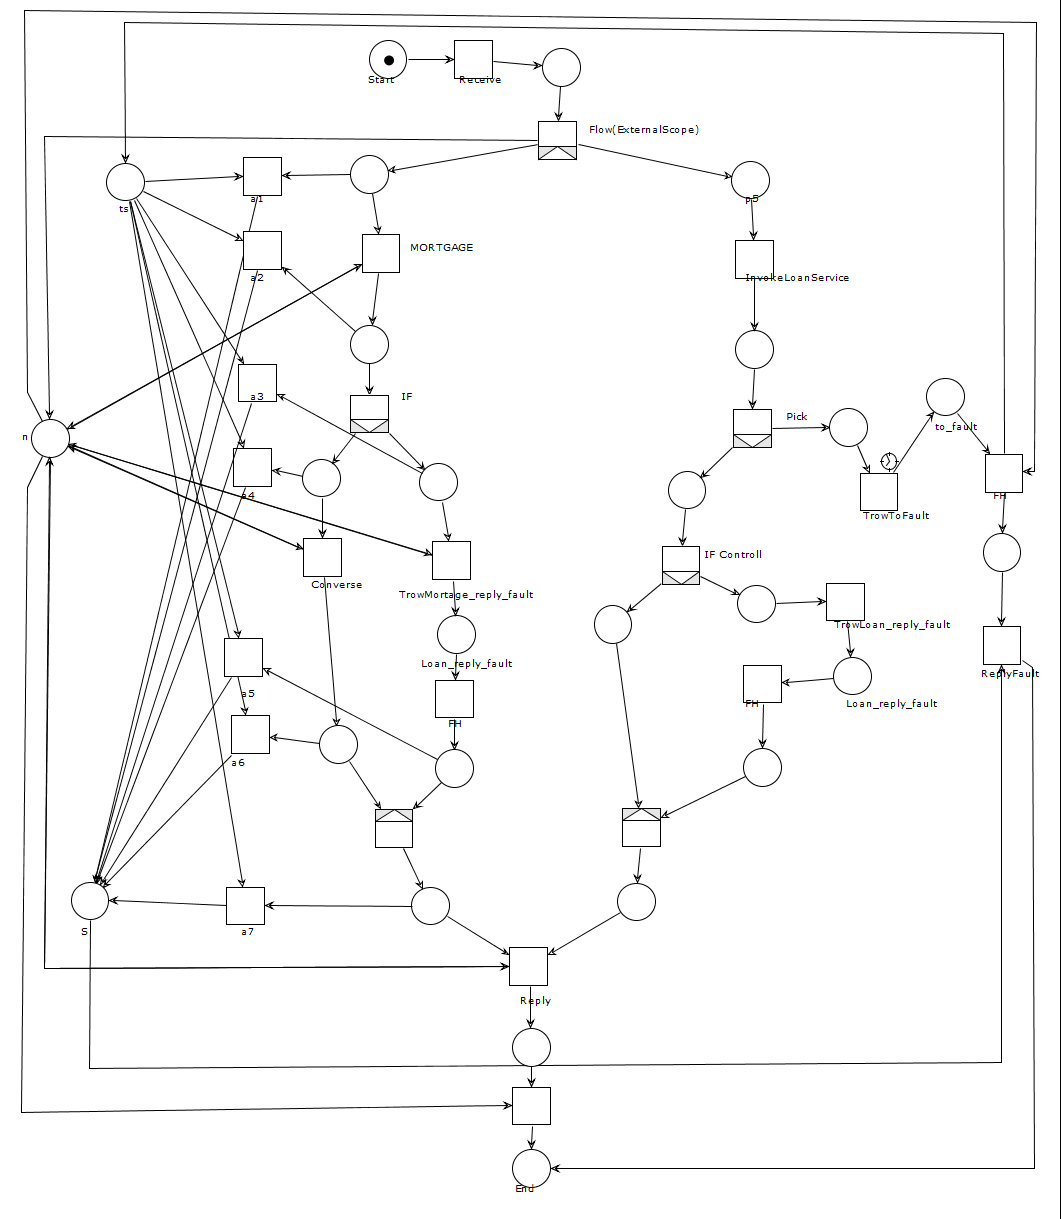
\includegraphics[width=1.1\columnwidth]{./pictures/WorkFlow.png} 
\caption[WorkFlow]{}  % The text in the square bracket is the caption for the list of figures while the text in the curly brackets is the figure caption
\label{fig:WorkFlow} 
\end{figure}



\end{document}